
\begin{frame}\frametitle{Doublet vs singlet}
\centering\myskip\scriptsize

MC simulated for {\cccolor singlet \T} with BR = 1/3 for
every decay mode

\begin{itemize}
\item Mixing between SM quarks and \T\ is {\cccolor left-handed} for singlets, {\cccolor right-handed} for doublets
\end{itemize}

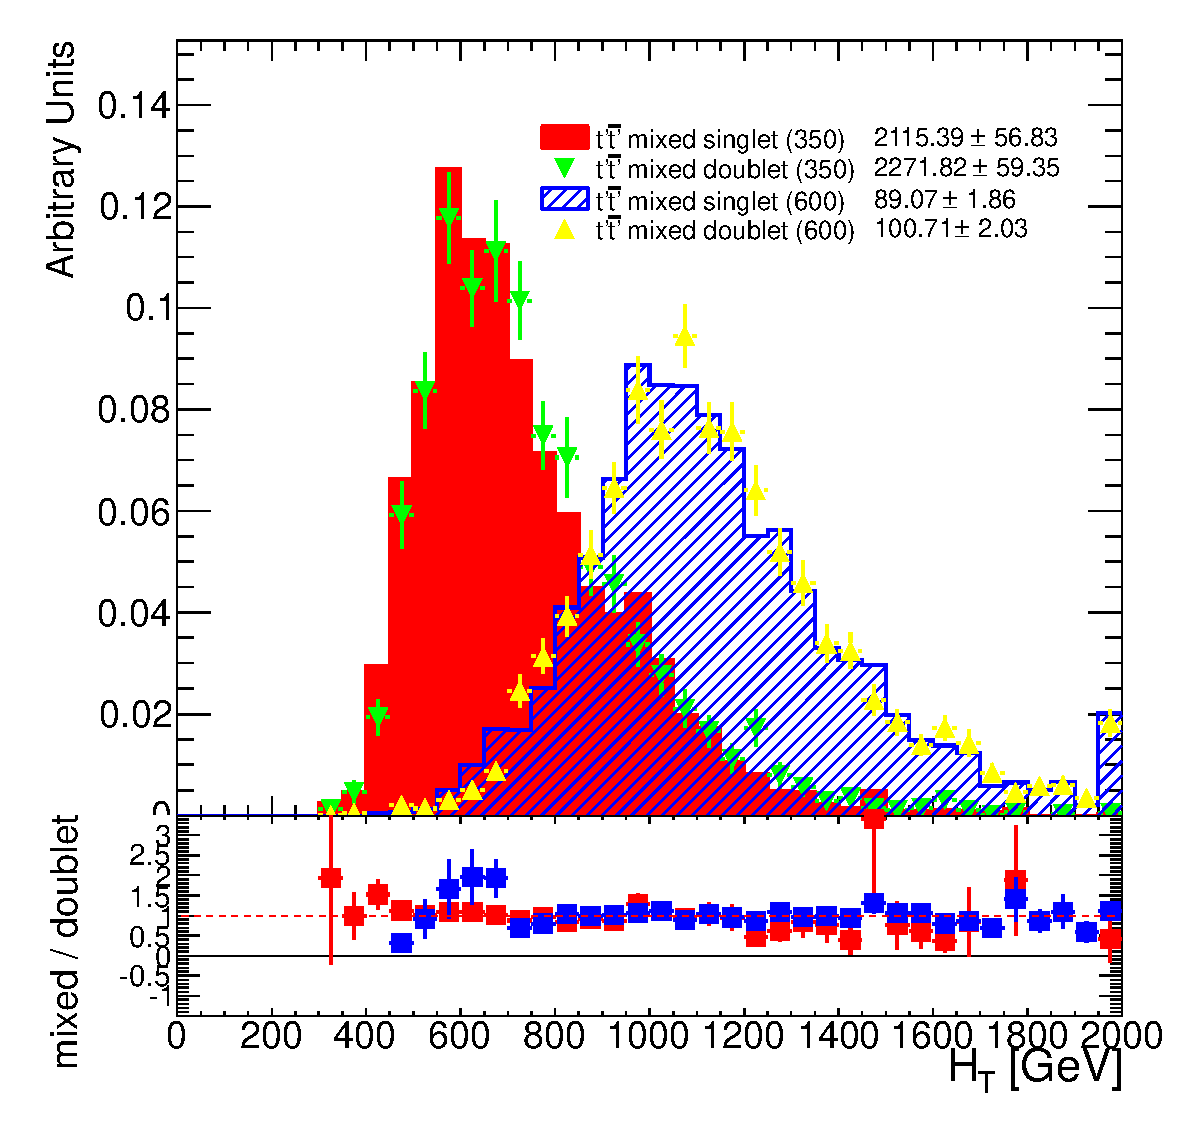
\includegraphics[width=0.45\textwidth]{pics/doubletcomp_HTAll_ELEMUON_6jetin3btagex_NOMINAL}
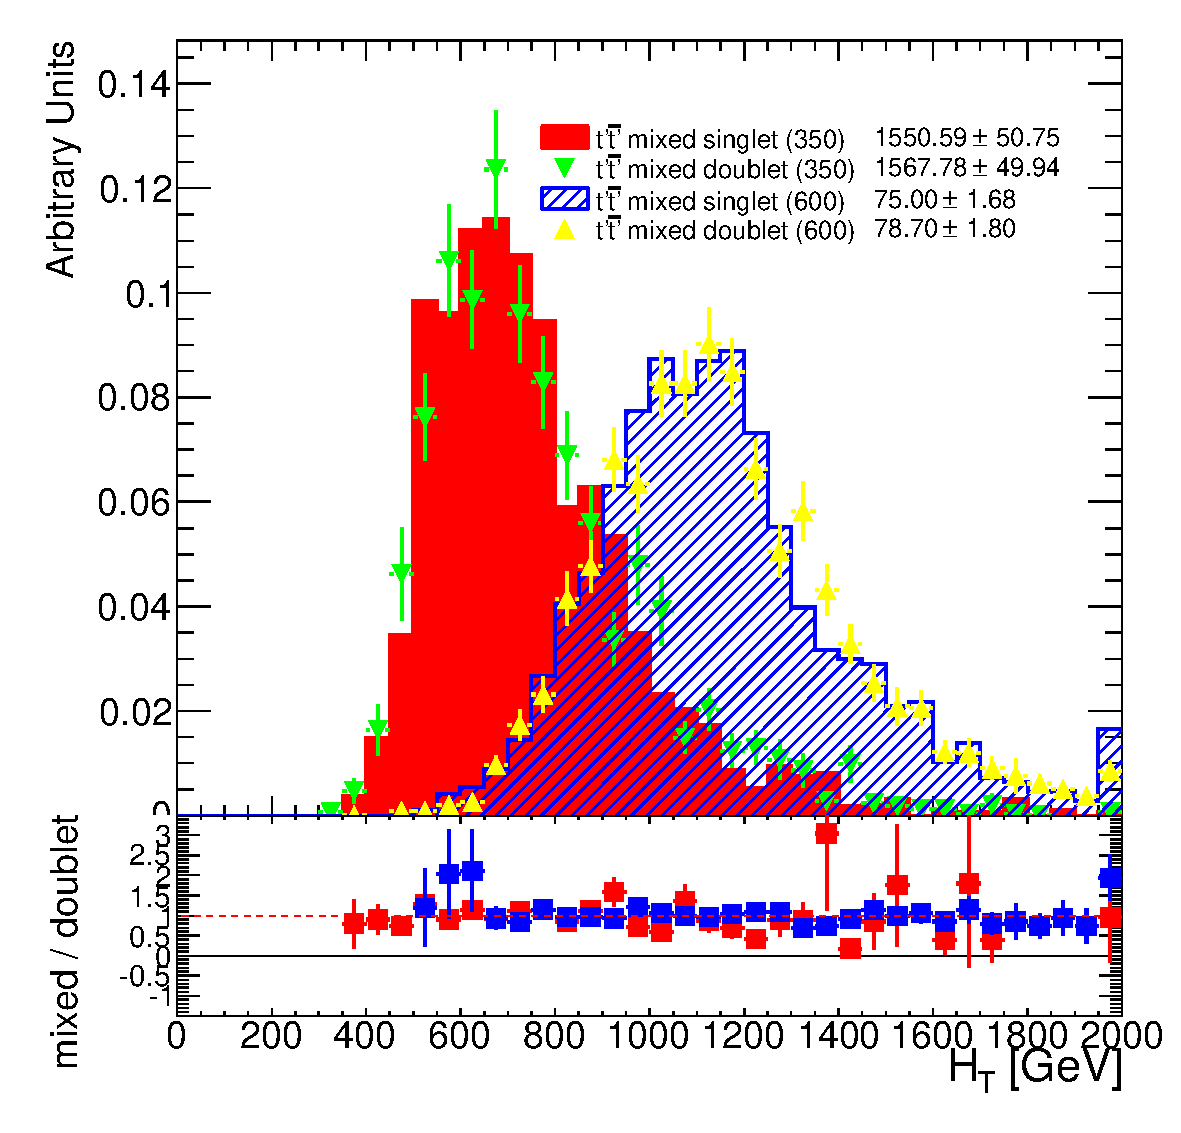
\includegraphics[width=0.45\textwidth]{pics/doubletcomp_HTAll_ELEMUON_6jetin4btagin_NOMINAL}

Discrepancies in yields below 5\% in \pchiv

\end{frame}



%%%%%%%%%%%%%%%%%%%%%%%%%
%%%
%%%%%%%%%%%%%%%%%%%%%%%%%
\begin{frame}\frametitle{Most relevant systematic uncertainties}
\centering\footnotesize


\resizebox{1.\textwidth}{!}{
\begin{tabular}{l*{10}{c}}
\toprule
 & \TTbar & $t\bar{t}$H (125) & $t\bar{t}$-HF & $t\bar{t}$-Light & $W$+jets & $Z$+jets & Single top & Diboson & $t\bar{t}$$V$ & Multijet\\
\midrule
Total [\%]& +21.9/-24.0 & +25.2/-30.0 & +57.3/-58.4 & +42.0/-44.1 & +60.0/-61.0 & +65.2/-66.2 & +31.7/-32.9 & +68.2/-70.2 & +37.6/-38.8 & +50.0/-50.0\\
\midrule
\multicolumn{10}{c}{Main contributions [\%]}\\
BTAGBREAK8 & +20.4/-22.7 & +18.7/-21.6 & +15.8/-17.8 & +12.2/-13.1 & +13.5/-15.0 & +13.0/-13.9 & +15.9/-17.8 & +22.0/-27.4 & +16.4/-18.6 & --\\
JES ``baseline'' & +3.1/-3.1 & +7.3/-7.3 & +10.5/-10.5 & +13.7/-13.7 & +18.1/-18.1 & +18.2/-18.2 & +19.9/-19.9 & +5.2/-5.2 & +8.4/-8.4 & --\\
ttbar iqopt2 & -- & -- & +6.9/-6.9 & +20.1/-20.1 & -- & -- & -- & -- & -- & --\\
ttbar ktfac & -- & -- & +7.5/-9.2 & +13.8/-17.0 & -- & -- & -- & -- & -- & --\\
ttbar qfac & -- & -- & +0.7/-0.7 & +1.6/-1.6 & -- & -- & -- & -- & -- & --\\
ttbarHF & -- & -- & +50.0/-50.0 & +13.0/-13.0 & -- & -- & -- & -- & -- & --\\
\bottomrule
\end{tabular}
}

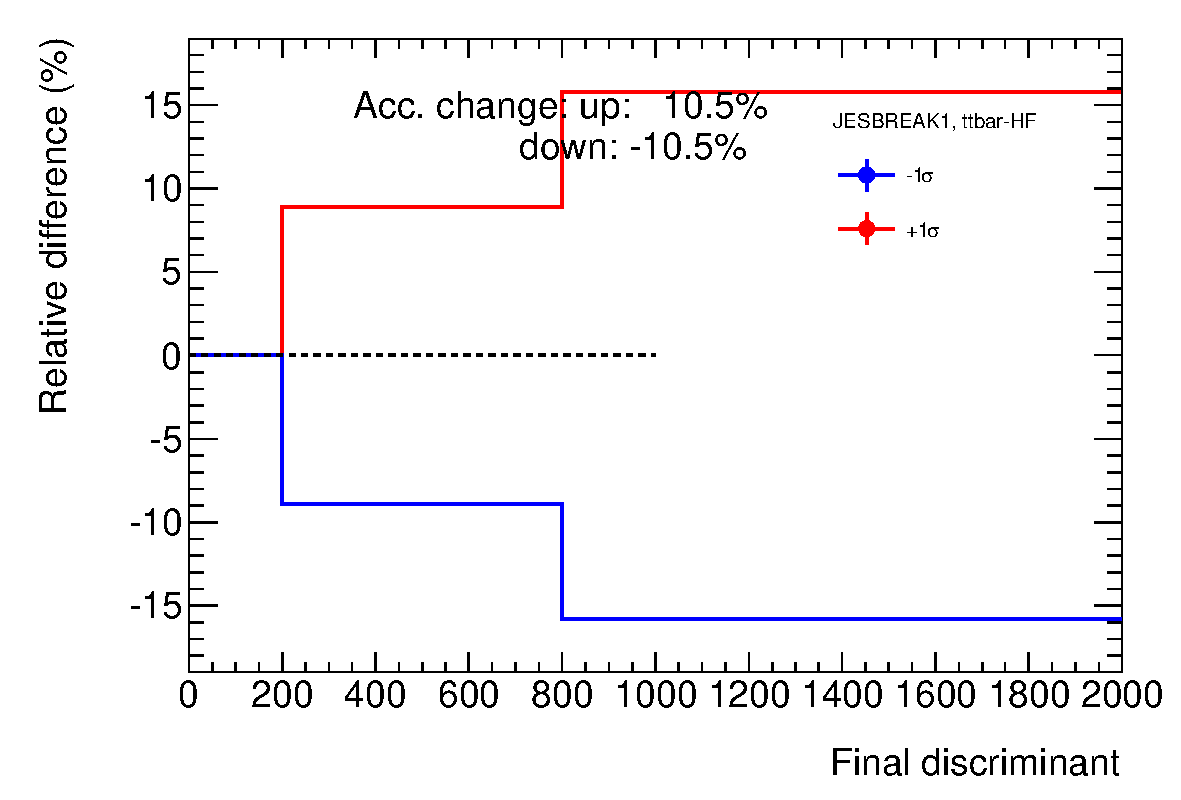
\includegraphics[width=.33\textwidth]{pics/6jetin4btagin_ELEMUON_ttbar-HF_JESBREAK1}
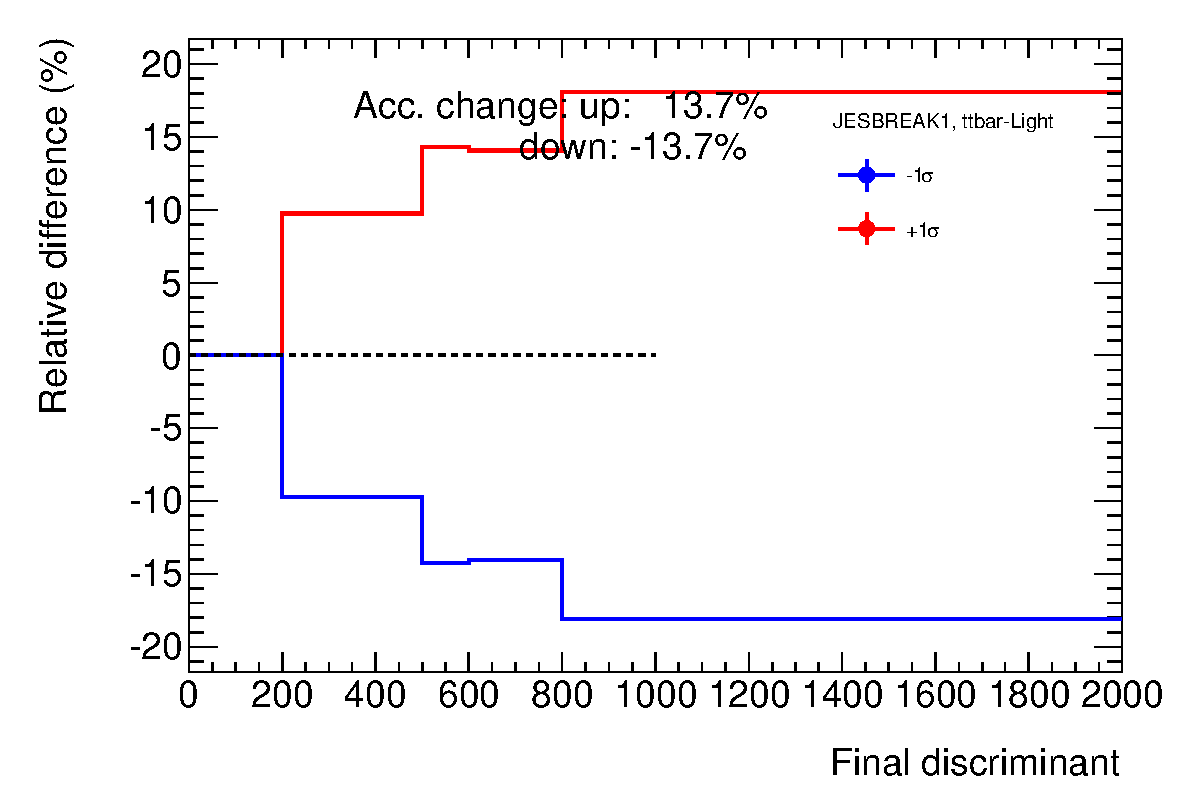
\includegraphics[width=.33\textwidth]{pics/6jetin4btagin_ELEMUON_ttbar-Light_JESBREAK1}


\end{frame}

